\documentclass[final]{beamer}

\usepackage[scale=1]{beamerposter} % Use the beamerposter package for laying out the poster

\usetheme{confposter} % Use the confposter theme supplied with this template

\setbeamercolor{block title}{fg=ngreen,bg=white} % Colors of the block titles
\setbeamercolor{block body}{fg=black,bg=white} % Colors of the body of blocks
\setbeamercolor{block alerted title}{fg=white,bg=dblue!50} % Colors of the highlighted block titles
\setbeamercolor{block alerted body}{fg=black,bg=dblue!10} % Colors of the body of highlighted blocks
% Many more colors are available for use in beamerthemeconfposter.sty

%-----------------------------------------------------------x   
% Define the column widths and overall poster size
% To set effecti ve sepwid, onecolwid and twocolwid values, first choose how many columns you want and how much separation you want between columns
% In this template, the separation width chosen is 0.024 of the paper width and a 4-column layout
% onecolwid should therefore be (1-(# of columns+1)*sepwid)/# of columns e.g. (1-(4+1)*0.024)/4 = 0.22
% Set twocolwid to be (2*onecolwid)+sepwid = 0.464
% Set threecolwid to be (3*onecolwid)+2*sepwid = 0.708

\newlength{\sepwid}
\newlength{\onecolwid}
\newlength{\twocolwid}
\newlength{\threecolwid}
\setlength{\paperwidth}{48in} % A0 width: 46.8in
\setlength{\paperheight}{36in} % A0 height: 33.1in
\setlength{\sepwid}{0.024\paperwidth} % Separation width (white space) between columns
\setlength{\onecolwid}{0.22\paperwidth} % Width of one column
\setlength{\twocolwid}{0.464\paperwidth} % Width of two columns
\setlength{\threecolwid}{0.708\paperwidth} % Width of three columns
\setlength{\topmargin}{-1.5in} % Reduce the top margin size
%-----------------------------------------------------------

\usepackage{graphicx}  % Required for including images

\usepackage{booktabs} % Top and bottom rules for tables

\usepackage{emoji} % Emoji :D

\usepackage{subcaption} % 2 images side by side
%-------------------------------------------s---------------------------------------------
%	TITLE SECTION 
%----------------------------------------------------------------------------------------

\title{A Proposed Framework for Acessing Bias on English Newspapers {\emoji[ios]{1F4F0}}} % Poster title

\author{Curado, Antonio  \&  Dahl, Morten} % Author(s)

\institute{Masters in Advanced Analytics @ Nova IMS} % Institution(s)

%----------------------------------------------------------------------------------------
%Elements:
%• abstract (1 2 sentences explaining your project)
%• description/intro (what is the problem? why is it hard? challenges?)
%• Methodology (how will you solve it)
%• methods you use (preprocessing you did, explain each method briefly, is it supervised/unsupervised, rule-based/ML, which assumptions )
%• metrics to evaluate you choose
%• results, highlighting what you want to show (make it visual / easy to understand) report metrics, videos or demos are a plus
%• show some examples of results
%• conclusions of results
%• future work: missing things from your work (work in progress) or future interesting work directions
%• make sure you cite every external code sources, datasets and papers you replicate/use (bibliography)
%• if you want and make the code publicly available write the link in the poster or QR code for people to use


\begin{center}
•
\end{center}\begin{document}

\addtobeamertemplate{block end}{}{\vspace*{2exs}} % White space under blocks
\addtobeamertemplate{block alerted end}{}{\vspace*{2ex}} % White space under highlighted (alert) blocks

\setlength{\belowcaptionskip}{2ex} % White space under figures
\setlength\belowdisplayshortskip{2ex} % White space under equations

\begin{frame}[t] % The whole poster is enclosed in one beamer frame

\begin{columns}[t] % The whole poster consists of three major columns, the second of which is split into two columns twice - the [t] option aligns each column's content to the top

\begin{column}{\sepwid}\end{column} % Empty spacer column

\begin{column}{\onecolwid} % The first column


%----------------------------------------------------------------------------------------
%	Abstract
%----------------------------------------------------------------------------------------

\begin{block}{Abstract}
    This project contributes to the detection of fake news by analysing bias in english newspapers. These Articles are grouped by topic and been undertaken a sentiment analysis to detect the bias and tendencies within each article. It results in a visualization, which shows the media bias per newspaper, topic and keyword.
\end{block}


%----------------------------------------------------------------------------------------
%	Motivation
%----------------------------------------------------------------------------------------

\begin{block}{Motivation {\emoji[ios]{1F4AA}}}

    The motivation from this project lays in the recent doubts on media neutrality. People tend to distrust the media and call serious newspapers "fake news", whereas dubious newspapers gain popularity. So this project aims to provide the following:
    \begin{itemize}
        \item provide a measure for biasness and tendentious media coverage
        \item create transparency which newspapers tend to publish more tendentious articles
        \item initial notions towards an automated biasness detection in media coverage
    \end{itemize}

\end{block}

%----------------------------------------------------------------------------------------
%	Methods
%----------------------------------------------------------------------------------------

\begin{block}{Methods}
    The methodology followed in this project is as followed: As a first step data was aquiered from a \textbf{web scrapping} aproach from which news articles are downloaded from the web representations of various well-known newspapers. The data was limited to the politics section of each newspaper. It was tried to pick a balanced selection of different politically located newspapers through a qualitative assessment.
    These articles were then filtered on keywords [e.g. "Trump", "Syria", "Brexit"] and been used to train a \textbf{LDA} model for topic detection. Simultaniously a \textbf{sentiment analysis} was carried out to measure the tendentious nature of each article. "A sentence on how it was done"
    Finally the results of both analysis were mapped and visualised in an interactive scatterplot. 
\end{block}
    
%----------------------------------------------------------------------------------------

\end{column} % End of the first column

\begin{column}{\sepwid}\end{column} % Empty spacer column

\begin{column}{\onecolwid} % Begin a column which is two columns wide (column 2)


%----------------------------------------------------------------------------------------
%	MATERIALS
%----------------------------------------------------------------------------------------

\begin{block}{Data Extraction}

    As a way to make the analysis relevant and up to date with the most current news topics
    it has been developed a new news dataset with the following porperties

    \begin{itemize}
        \item Built a dataset with over \textbf{70.000} news articles
        \item Scraped over \textbf{19} newspapers for over \textbf{2} weeks
        \item With an average of \textbf{3.600} news articles per newspaper
    \end{itemize}

    \hfill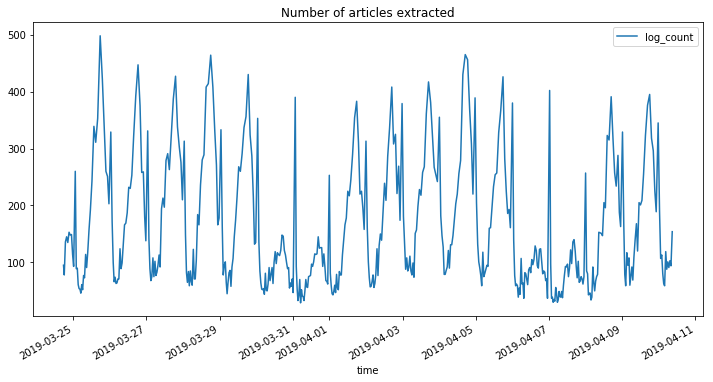
\includegraphics{log_extraction.png}\hspace*{\fill}

    The dataset was build only using the newspapers3k python package

\end{block}

%----------------------------------------------------------------------------------------
%	MATHEMATICAL SECTION
%----------------------------------------------------------------------------------------

\begin{block}{LDA Analysis}

    The LDA (Latent Dirichlet Allocation) analysis aims to detect topics within all articles. We trained a model for each partition of the dataset. The dataset was partitioned based on a specific keyword (e.g. Trump) in order to have a meaningful filter. Otherwise the dataset would be too big to analyse each detected topic. This algorithm takes three \textit{hyperparameters}: number of topics, alpha and eta. All of these parameters were finetuned for each of the three trained models. The coherence score served as a measure for this assessment. \linebreak
    
    \begin{table}    
    \begin{tabular}{c c c c}
    \hline
    KeyWord & Topics & Alpha & Eta  \\ [0.5ex]
    \hline\hline
    "Trump" & 14 & 0.01 & 0.01 \\
    "Brexit" & 6 & 0.01 & 0.01 \\
    "Syria" & 6 & 0.6 & 0.2 \\
    \end{tabular}
    \caption{Parameters for LDA models}
    \end{table}
    
     The result of this analysis is a mapping for each article in order to make them comparable. Each topic is represented as a concatination of words assigned with a probability. In the example topic shown below one can understand by examining the words, that the topic is about Trump and the wall to mexico. \linebreak
     
     \textit{0.033*"border" + 0.016*"mexico" + 0.016*"trump" \\
    + 0.010*"immigration" + 0.008*"states" + 0.008*"united" \\
    + 0.008*"president" + 0.007*"illegal" + 0.007*"migrants" \\
    + 0.006*"people"}


       \end{block}

    \begin{block}{Sentiment Analysis}

        Another way to search for is to analyse the sentiment which each newspaper looks at a topic.
        With a help of a word dictionary quantifiyng the polatiy of each word, the polarity for each article has been calculated.\cite{vader}

    \end{block}

\end{column} % End of the first column


\begin{column}{\sepwid}\end{column} % Empty spacer column

\begin{column}{\twocolwid} % The third column

%----------------------------------------------------------------------------------------
%	TRUMP
%----------------------------------------------------------------------------------------

\begin{block}{Trump}

\begin{columns}[onlytextwidth]
    \begin{column}{.45\textwidth}
        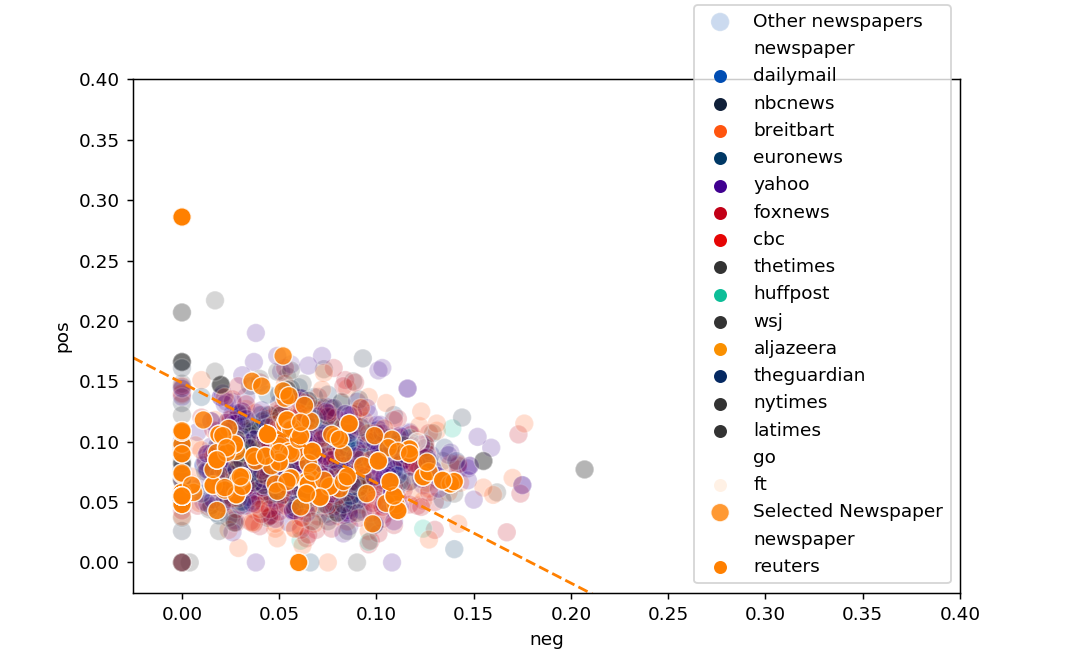
\includegraphics[width=0.8\linewidth]{poster/trump_11_reuters.png} 
    \end{column}
    \begin{column}{.55\textwidth}
        This is an example plot of the analysis of a topic containing the keyword "Trump". The topic covers the investigation done by Robert Mueller regarding the involvement of russia in the presidential election in 2016. The news agency /textbf{reuters} apparently covered this topic in a slight negative manner, but still more or less balanced. Each point in the scatter represent an article, whereas the x-axis shows the negative score and the y-axis the positive score. In this framework a rather lower score on both axis means less usage of \textit{tendencious} words.
    \end{column}
\end{columns}

\end{block}

%----------------------------------------------------------------------------------------
%	BREXIT
%----------------------------------------------------------------------------------------

\begin{block}{Brexit {\emoji[windows]{1F1E7}}}


    \begin{columns}[onlytextwidth]
        \begin{column}{.55\textwidth}
            This plot shows the coverage of the topic, that the brexit will impact the global trade. The newspaper \textbf{the times} covers this topic apparently more ambivalent. The sparse distribution of points suggest, that the coverage of the different articles have different tones.
        \end{column}
        \begin{column}{.45\textwidth}
            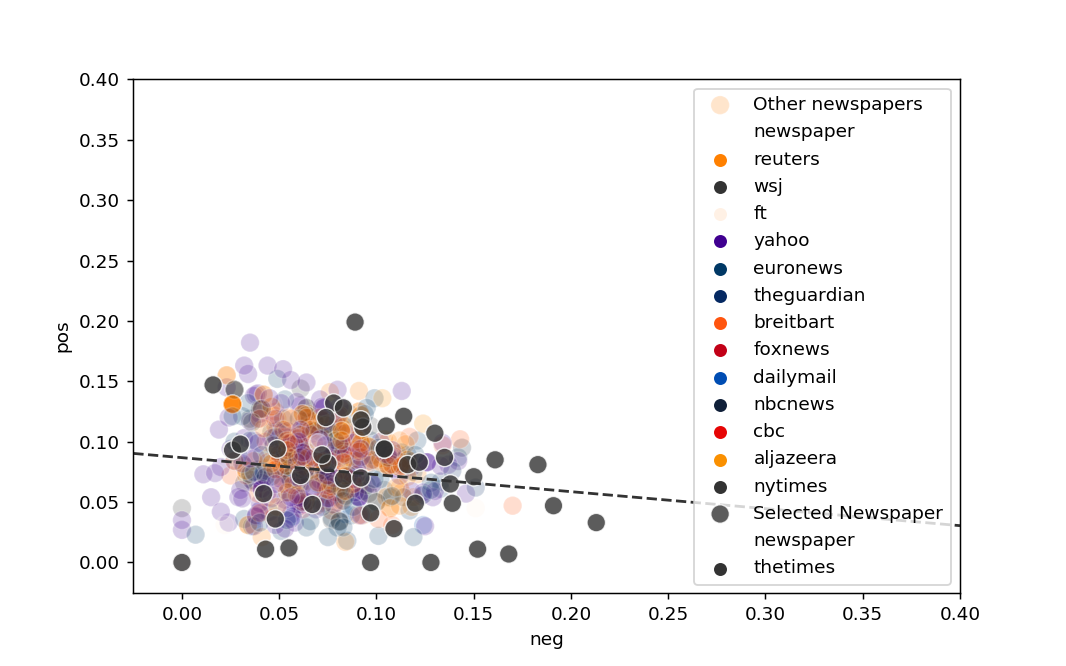
\includegraphics[width=0.8\linewidth]{poster/brexit_5_thetimes.png} 
        \end{column}
    \end{columns}

\end{block}

%----------------------------------------------------------------------------------------
%	SYRIA
%----------------------------------------------------------------------------------------

\begin{block}{Syria}
    \begin{columns}
        \begin{column}{.45\textwidth}
            \begin{figure}
                \centering
                \begin{minipage}{.5\textwidth}
                \centering
                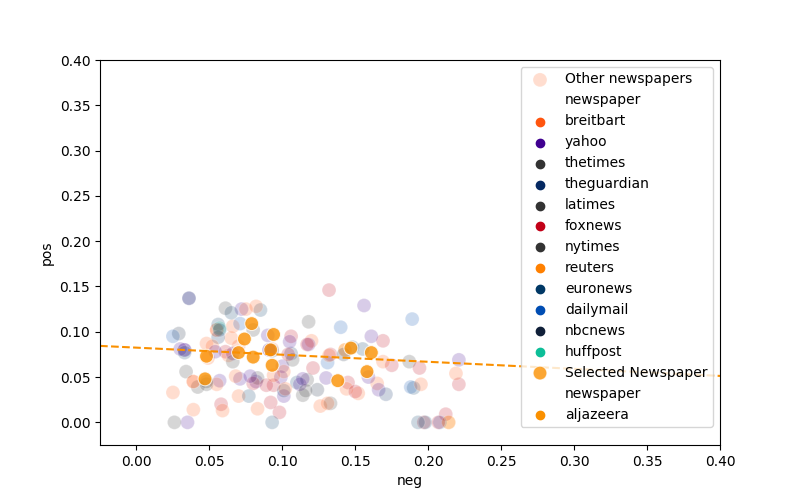
\includegraphics[width=\linewidth]{poster/syria_5_al.png}
                \captionof{figure}{Al Jazeera}
                \label{fig:test1}
                \end{minipage}%
                \begin{minipage}{.5\textwidth}
                \centering
                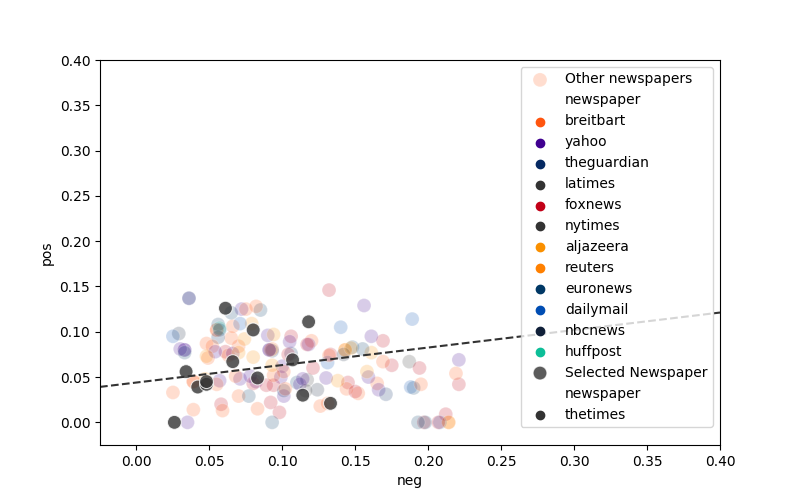
\includegraphics[width=\linewidth]{poster/syria_5_thetimes.png}
                \captionof{figure}{The Times}
                \label{fig:test2}
                \end{minipage}
            \end{figure}
        \end{column}

        \begin{column}{.55\textwidth}
            The two plots show how articles from the Al Jazeera and The Times newspapers compare to each other, on a positivity/negativity scale.
            Both are measured on the topic 5 which contains as most frequent keywords:  \\
            From this one could possibly infer that when Al Jazeera publishes on the topic, it takes more serious and possible more negative approach to it.\\
            Never the less, these are only possible assumptions that the framework helps to clarify. Each article would be needed to be read in details to derive further conclusions
        \end{column}
    \end{columns}
\end{block}

%---------------------------------------------------------------------------------------
%	FUTURE WORK & Conclusion
%----------------------------------------------------------------------------------------

\begin{block}{Conclusion {\emoji[ios]{1F64F}}}
    Measuring bias is a very subjective task. 
    Usually computers have a hard time executing subjective tasks. 
    The framework developed does not aim to automate bias detection but 
    rather to empower humans with summarization capabilites otherwise not possible.
    From the three example analysis above shown, it is possible to validate the usefullness of the framework proposed on a hard topic as bias detection.
    As news generation gets automated, as is the case of fakenews(needs reference), the methods of flaging them also require modern digital frameworks.
    This analysis and framework takes another step in this direction.

\end{block}


\begin{block}{Future Work {\emoji[ios]{1F64F}}}

    As previously mentioned this project aims to set a staring framework for discusion on automated detection of bias. 
    As so there is much further work to be done, mainly on 5 different areas:

    \begin{itemize}
        \item Increase the number of newspapers and find a method to select the same number of articles for each one
        \item Extrapolate the work to different regions and languages
        \item Automate topic detection 
        \item Build a ML/Rule based algorithm to flag possible high bias on articles
        \item Apply sliding window mechanimns to track changes in sentiment towards selected topics
    \end{itemize}

\end{block}


%----------------------------------------------------------------------------------------
%	REPO
%----------------------------------------------------------------------------------------

\begin{block}{ {\emoji[ios]{1F4BB}}}
    \begin{thebibliography}

        \bibitem{vader}
          Hutto, C.J. and Gilbert, Eric,
          \emph{ A Parsimonious Rule-based Model for Sentiment Analysis of Social Media Text},
          Proceedings of the 8th International Conference on Weblogs and Social Media, ICWSM 2014,
          2015.
    \end{thebibliography}
    \vspace{8mm}
    The project was possible with the great work done in the newspaper3k, nltk and gensim python libraries

    \small{\rmfamily{All code can be easily accessed in \href{https://github.com/morten-novaims/Text_Mining_HW}{github.com/morten-novaims/Text\_Mining\_HW}}} \\
    
    \end{block}

%----------------------------------------------------------------------------------------

\end{column} % End of the third column

\end{columns} % End of all the columns in the poster

\end{frame} % End of the enclosing frame

\end{document}